%% ================================================================
%% # DBIS Databases Data Analysis Project Part 0 Template
%% 
%% Template for students to hand-in their databases exercise solutions.
%% 
%% [Databases and Information Systems Group](https://dbis.dmi.unibas.ch/)
%%
%% ## Usage
%% 
%% Fill in the required fields and write your submission
%%
%% ## Issues
%%
%% See dbisdbprojp0.sty for further information.
%% ================================================================
\documentclass{article}
\usepackage{dbisdbprojp0}
\usepackage{url}




%% ================================================================
%%
%% General Information
%%
%% ================================================================
%%
%% Add your information here
\course       {Databases}
\semester     {Autumn 2020}
\title        {Data Analysis Project\\P1: Schema Integration}
\subtitle     {Visualizing Traffic density data and comparing them to air pollution- and meteorological data in Basel, London and Los Angeles}
\studenta     {Pascal Kunz}
\studentb     {Etienne Mettaz}
%\studentc     {Alan Turing}


%% ================================================================
%%
%% Common Packages
%%
%% ================================================================
%%
%% Useful common packages for this course

%% Drawing everything, with lots of libraries
\usepackage{tikz}
%% A library providing ER prefabs
\usetikzlibrary{er}

%% ================================================================
%%
%% Custom Packages
%%
%% ================================================================
%%
%% Add custom packages below:
%%


\begin{document}
%% Required for the title
\printfront
%% ================================================================
%%
%% Description
%%
%% ================================================================

\section{Entities and their attributes}

We will specify the entities in their as is state and provide an exemplary tuple for each entity.

\subsection{UTD19}

\begin{tabular}{ |p{5cm}| p{5cm}|  }
\hline
 Entitiy: UTD 19 & Example\\
 \hline
Attributes: \uline{Day} & 2017-05-06\\
\uline{Interval}& 0 \\
\uline{City}& augsburg\\
 Detid & 06.X-2li\\
 Flow & 12\\
 Occupancy & 0\\
 Error & 1\\
 Speed & <Null>\\
 \hline
\end{tabular}

Exemplary Tuple, in order of the Table above:




\subsection{Detectors}

\begin{tabular}{ |p{5cm}| p{5cm}| }
\hline
 Detectors & Example\\
 \hline
 \uline{detid} & U1-52G\\
length& 0.1960.\\
 pos & 0.0055\\
 fclass& secondary\\
 road& Gögginger Straße\\
limit& 50\\
 citycode& augsburg\\
  lanes& 1\\
linkid& 72\\
 long& 10.8895527\\
  lat& 48.359957\\
 \hline
\end{tabular}\\






\subsection{Links}

\begin{tabular}{ |p{5cm}| p{5cm}|  }
\hline
 Links & Example\\
 \hline
 long & 10.8910158\\
lat& 48.3610789\\
 \uline{order}& 1\\
 piece& 1\\
 \uline{linkid}& 0\\
group& 0.1\\
 \uline{citycode}& augsburg\\
 \hline
\end{tabular}\\



\begin{tabbing}
    Links (10.8910158,48.3610789,1,1,0,0.1,augsburg

)\\
\end{tabbing}

\subsection{Air quality Basel Feldbergstrasse}

\begin{tabular}{ |p{8cm}| p{5cm}| }
\hline
 AQ Basel Feldbergstrassse & Example\\
 \hline
 \uline{Location} & Basel\\
 \uline{Datum/Zeit} & 2001-04-24T05:00:00+00:00\\
timestamp text& 2001-04-24 06:00:00\\
 PM10 (Stundenmittelwerte [µg/m³])& 33.624 \\
 PM2.5 (Stundenmittelwerte [µg/m³])& 17.911\\
 NO2 (Stundenmittelwerte [µg/m³])& 34.481\\
geo point 2d  & 47.5670167,7.5925446\\
 \hline
\end{tabular}\\





\subsection{Air quality Basel St. Johannsplatz}

\begin{tabular}{ |p{8cm}| p{5cm}| }
\hline
 AQ Basel St Johannsplatz & Example\\
 \hline
  \uline{Location} & Basel\\
 \uline{Datum/Zeit} & 2015-09-15T07:00:00+00:00\\
timestamp text& 2015-09-15 08:00:00 \\
 PM10 (Stundenmittelwerte [µg/m³])&9.091 \\
 PM2.5 (Stundenmittelwerte [µg/m³])& 1.425
\\
 NO2 (Stundenmittelwerte [µg/m³])& 3.892\\
geo point 2d & 47.5659354,7.58192\\
 \hline
\end{tabular}\\

Exemplary Tuple, in order of the Table above:

\begin{tabbing}
    AQ Basel Feldbergstrassse (2015-09-15T07:00:00+00:00,2015-09-15 08:00:00,9.091,,3.892,"47.5659354,7.58192")



)\\
\end{tabbing}

\subsection{Air quality Basel Chrischona}

\begin{tabular}{ |p{8cm}| p{5cm}|  }
\hline
 AQ Basel Chrischona & Example\\
 \hline
  \uline{Location} & Basel\\
 \uline{Datum/Zeit} & 2003-06-04T03:00:00+00:00\\
timestamp text & 2003-06-04T04:00:00+00:00\\
 O3 (Stundenmittelwerte [µg/m³])& 114.265\\
geo point 2d & 47.5717,7.6870833\\
 \hline
\end{tabular}\\


\subsection{Air qualitiy London}

As all the subfiles need to be downloaded for one site at a time from London Air: \url{https://www.londonair.org.uk/london/asp/datadownload.asp} but all have the same format, we will list one example for London upper Thames street.\\

\begin{tabular}{ |p{8cm}| p{5cm}|  }
\hline
 AQ London upper thames street & Example\\
 \hline
 \uline{Location} & London\\
 \uline{Site} & CT8 \\
Species &PM10\\
 \uline{ReadingDateTime} & 01/01/2015 00:00\\
 Value & 44 \\
Units & ug/m3\\
Provisional or Ratified & R\\
 \hline
\end{tabular}\\




\subsection{Air Quality Los Angeles}


\begin{tabular}{ |p{8cm}| p{5cm}|  }
\hline
 AQ US hourly & Example\\
 \hline
 \uline{State Code} & 1\\
 \uline{County Code} & 3\\
\uline{Site Num}&  10\\
 \uline{Parameter Code}& 44201\\
 POC& 1\\
Latitude& 30.497477999999997\\
Longitude& -87.880258\\
 Datum& NAD83\\
 Parameter Name& Ozone\\
\uline{Date Local}& 2017-03-01 \\
\uline{Time Local}& 04:00\\
 Date GMT& 2017-03-01\\
 Time GMT& 10:00\\
Sample Measurement& 0.022000000000000002\\
Units of Measure& Parts per million\\
MDL& 0.005\\
Uncertainty&  \\
 Method Type& FEM\\
Method Code& 87\\
Method Name& INSTRUMENTAL - ULTRA VIOLET ABSORPTION\\
State Name& Alabama \\
County Name& Baldwin\\
Date of Last Change& 2017-05-18\\
 \hline
\end{tabular}\\





\subsection{weather Basel}


\begin{tabular}{ |p{8cm}| p{5cm}|   }
\hline
 weather Basel & Example\\
 \hline
 \uline{City Name} & Basel
\\\uline{timestamp} & 20101020T0000
\\Basel Temperature [2 m elevation corrected]& 8.190529
\\Basel Relative Humidity [2 m] &87.0
\\Basel Mean Sea Level Pressure [MSL] &1009
\\Basel Precipitation Total& 0.0
\\Basel Snowfall Amount & 0.0
\\Basel Cloud Cover Total& 100.0
\\Basel Cloud Cover High [high cld lay]& 0.0
\\Basel Cloud Cover Medium [mid cld lay]&100.0
\\Basel Cloud Cover Low [low cld lay]& 100.0
\\Basel Wind Speed [10 m]& 29.519999
\\Basel Wind Direction [10 m]& 16.179985\\
 \hline
\end{tabular}\\



\subsection{weather London, Los Angeles (Same format two different CSV files)}


\begin{tabular}{ |p{8cm}| p{6cm}|  }
\hline
 weather London, Los Angeles & Example\\
 \hline
\uline{City Name} & London or LA (depending on file)
\\\uline{date} & 2008-07-01
\\\uline{time} & 0
\\tempC& 17
\\windspeedKmph& 1
\\weatherDesc& Clear
\\precipMM&0
\\precipInches& 0
\\humidity& 71
\\pressureMB& 1013
\\pressureInches& 30
\\cloudcover& 0
\\DewPointC& 16
\\WindChillC& 21
\\FeelsLikeC&21 \\
 \hline
\end{tabular}\\

\newpage

\subsection{Basel MVI)}


\begin{tabular}{ |p{8cm}| p{6cm}|  }
\hline
 Basel MVI & Example\\
 \hline
 \uline{SiteCode}& 235\\
    SiteName&  235 A3-A35 \\
    \uline{DirectionName}& von Frankreich \\
    \uline{LaneCode}& 1\\
    LaneName& Spur 1\\
    \uline{Date}& 21.08.2014\\
    \uline{TimeFrom}& 01:00\\
    TimeTo& 02:00\\
    ValuesApproved& - \\
    ValuesEdited& -\\
    TrafficType& MIV \\
    Total& 58\\
    MR& 58\\
    PW& 0\\
    `PW+`& 0\\
    Lief& 0\\
    `Lief+`& 0\\
    `Lief+Aufl.`& 0\\
    LW &0 \\
    `LW+`& 0 \\
    Sattelzug & 0\\
    Bus& 0 \\
    andere & 0\\
    DateTimeFrom & 2014-08-21 00:00:00+00:00\\
    DateTimeTo   & 2014-08-21 01:00:00+00:00\\
    Year     & 2014\\
    Month     & 8\\
    Day         & 21\\
    Weekday       & 3\\
    HourFrom     & 1\\
 \hline
\end{tabular}\\


\newpage






\section{ER-Diagram}

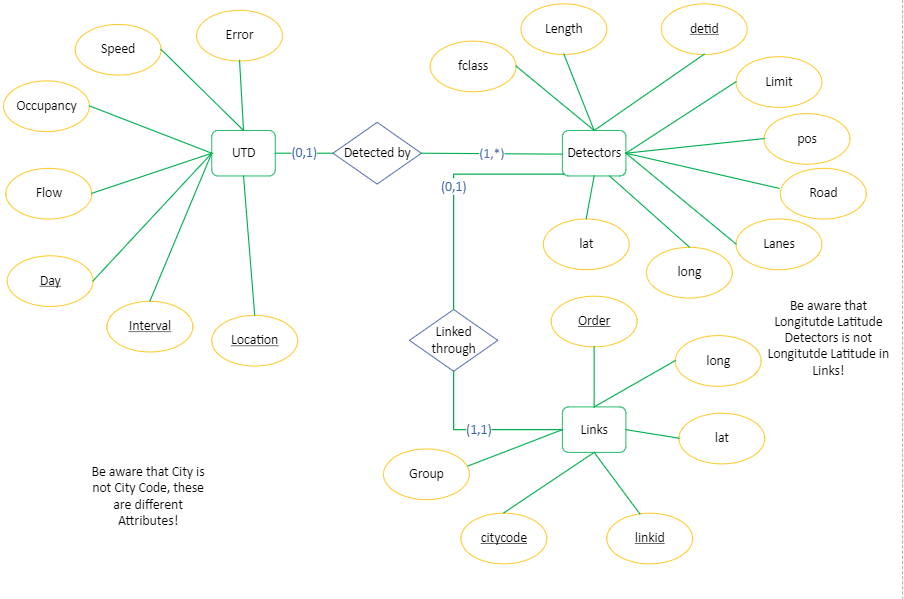
\includegraphics[scale=0.5]{first.png}\\
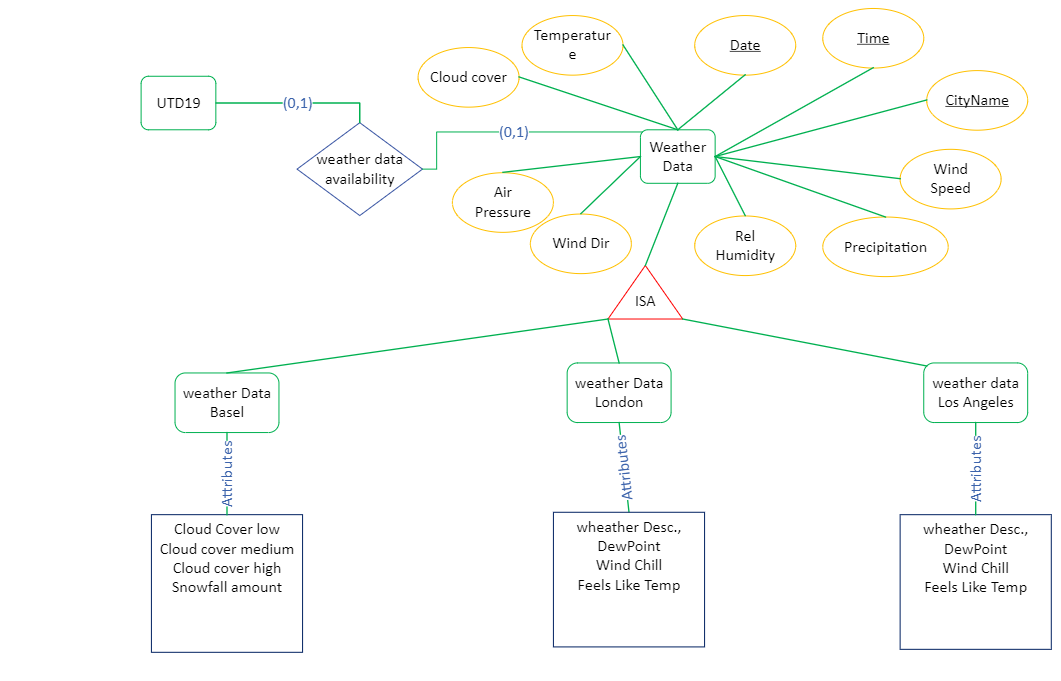
\includegraphics[scale=0.5]{second.png}\\
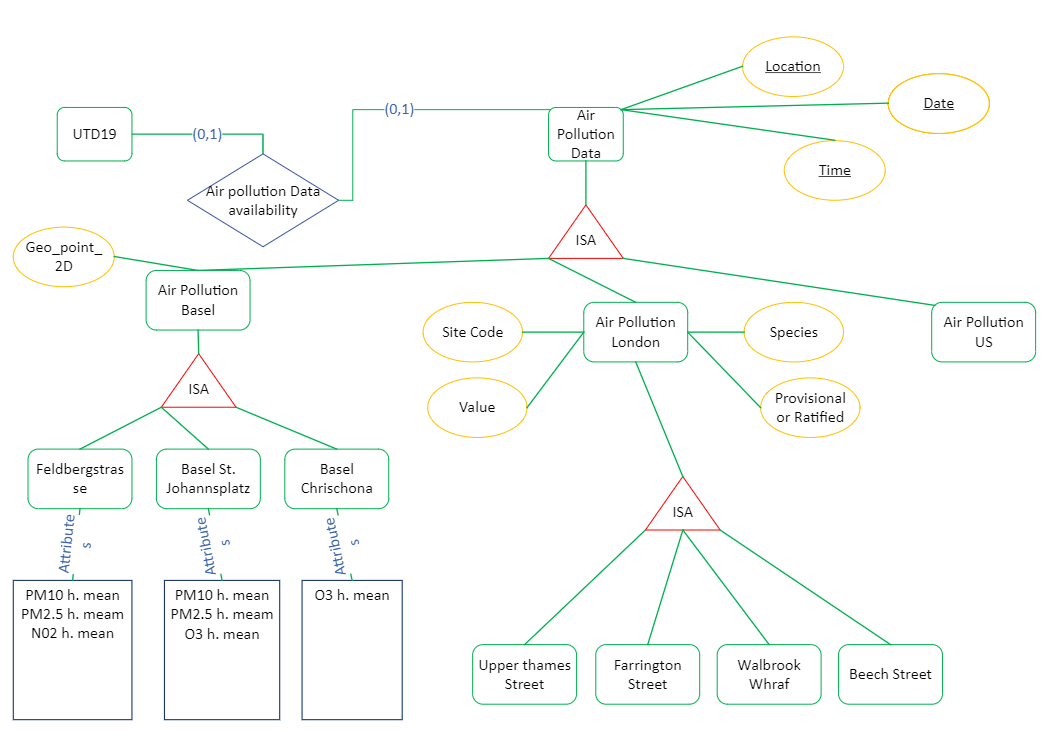
\includegraphics[scale=0.6]{third.png}
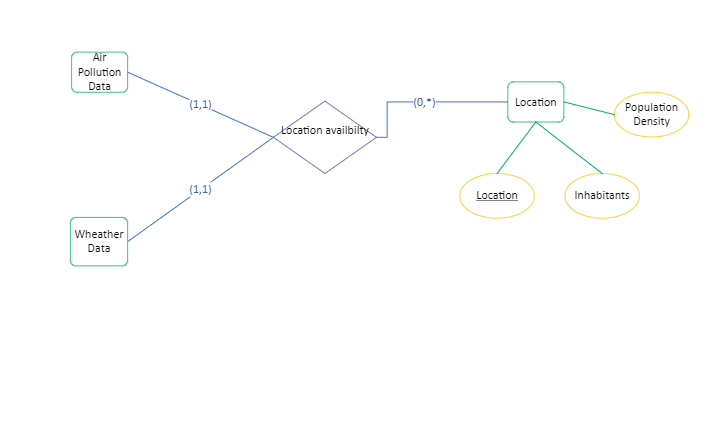
\includegraphics[scale=0.6]{fourth.png}
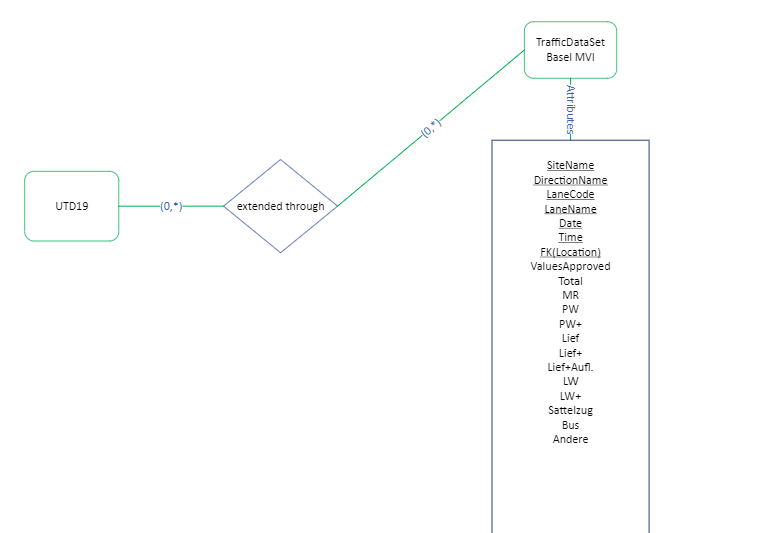
\includegraphics[scale=0.6]{fifth.png}



\section{logical scheme}
\begin{center}
\begin{tabbing}
    UTD19 \qquad\qquad\qquad\= (\uline{Day, Interval, City},  \uwave{DetID}, Flow, Occupancy, Speed)\\\\
    Detectors \> (\uline{DetID}, \uwave{LinkID, City Code}, Length, Road, Speed Limit, Position, Lanes, Longitude, Latitude)\\\\
    %Detected by \> (\uline{\uwave{DetID, Interval, Day}}, \uwave{LinkID, City Code})\\
    Links \> (\uline{LinkID, City Code},Order, Latitude, Longitude, Group)\\\\
    
    
    
    
    
    Weather Data \> (\uline{Date, Time, CityName},  \uwave{Day, Interval, City}, Cloud Cover, Temperature, Rel Humidity,\\ \> Precipitation, Wind Speed)\\\\
    %W. D. Availability \> (\uline{\uwave{Date, Time, Location}, \uwave{Det ID, Interval}})\\
    
    W. D. Basel \> (\uline{Date, Time, CityName},  \uwave{Day, Interval, City},Wind Direction, Cloud Cover low,\\ \>  Cloud Cover medium,Cloud Cover 		High, Snowfall amount, Air pressure,\\ \> Cloud Cover, Temperature, Rel Humidity, Precipitation, Wind Speed)\\\\
    W. D. London \> (\uline{Date, Time, CityName}, \uwave{Day, Interval, City}, Wind Chill,Heat index, Snow, Snow Depth\\ \>, Wind Gust, Visibility, Conditions, Cloud Cover, Temperature, Rel Humidity,\\ \> Precipitation, Wind Speed)\\\\
    W. D. Los Angeles \> (\uline{Date, Time, CityName}, \uwave{Day, Interval, City}, Wind Chill,Heat index, Snow, Snow Depth\\ \>, Wind Gust, Visibility, Conditions, Cloud Cover, Temperature, Rel Humidity,\\ \> Precipitation, Wind Speed)\\
    \\
    
    %Air Pol. Data avail. \> (\uline{\uwave{Location, Date, Time}, \uwave{DetID, Interval}})\\
    Air Pollution Data \> (\uline{Location, Date, Time}, \uwave{Day, Interval, City})\\
    Air Pollution Basel \> (\uline{Location, Date, Time}, \uwave{Day, Interval, City},  Geo Point 2D)\\\\
    Feldbergstrasse \> (\uline{Location, Date, Time},\uwave{Day, Interval, City}, Geo Point 2D, PM10 h. mean,\\ \> PM2.5 h. mean, NO2 h. mean)\\\\
    St. Johannsplatz \> (\uline{Location, Date, Time}, \uwave{Day, Interval, City} Geo Point 2D, PM10 h. mean,\\ \> PM2.5 h. mean, O3 h. mean)\\\\
    Chrischona \> (\uline{Location, Date, Time}, \uwave{Day, Interval, City} Geo Point 2D, O3 h. mean)\\
    \\
    Air Pollution London \> (\uline{Location, Date, Time}, \uwave{Day, Interval, City} Site Code, Value, Species, Provisional or Ratified)\\\\
    Upper thames Street \> (\uline{Location, Date, Time}, \uwave{Day, Interval, City} Site Code, Value, Species, Provisional or Ratified)\\\\
    Farrington Street \> (\uline{Location, Date, Time}, \uwave{Day, Interval, City}, Site Code, Value, Species, Provisional or Ratified)\\\\
    Walbrook Whraf \> (\uline{Location, Date, Time}, \uwave{Day, Interval, City} Site Code, Value, Species, Provisional or Ratified)\\\\
    Beech Street \> (\uline{Location, Date, Time}, \uwave{Day, Interval, City} Site Code, Value, Species, Provisional or Ratified)\\\\
            
    \\
    Air Pollution US \> (\uline{Location, Date, Time}, \uwave{Day, Interval, City}, State Code, County Code, Site Number,\\ \> Parameter Code, Paraneter Name, POC, Latitude, Longitude, MDL,\\ \> Uncertainity, Units of measurement)\\\\
    Air Pol. US $SO_{2}$  \> (\uline{Location, Date, Time}, \uwave{Day, Interval, City}, State Code, County Code, Site Number,\\ \> Parameter Code, Paraneter Name, POC, Latitude, Longitude, MDL,\\ \> Uncertainity, Units of measurement)\\\\
    Air Pol. US $CO$  \> (\uline{Location, Date, Time}, \uwave{Day, Interval, City}, State Code, County Code, Site Number,\\ \> Parameter Code, Paraneter Name, POC, Latitude, Longitude, MDL,\\ \> Uncertainity, Units of measurement)\\\\
    Air Pol. US $O_3$  \> (\uline{Location, Date, Time}, \uwave{Day, Interval, City}, State Code, County Code, Site Number,\\ \> Parameter Code, Paraneter Name, POC, Latitude, Longitude, MDL,\\ \> Uncertainity, Units of measurement)\\\\
    Air Pol. US $NO_2$  \> (\uline{Location, Date, Time}, \uwave{Day, Interval, City}, State Code, County Code, Site Number,\\ \> Parameter Code, Paraneter Name, POC, Latitude, Longitude, MDL,\\ \> Uncertainity, Units of measurement)\\\\
    
    
    ExtendedThrough \> (City, Interval, Day,

SiteName,

DirectionName,

LaneCode
,
LaneName,
\\ \>

Date,

TimeFrom,

Time To,

DateTimeFrom,

DateTimeTo,

Year,

)\\\\

    Basel MVI \> (PrimaryKeys(City, Interval, Day,

SiteName,

DirectionName,

LaneCode
,
LaneName,
\\ \>

Date,

TimeFrom,

Time To,

DateTimeFrom,

DateTimeTo,

Year),

\\ \> ValuesApproved,

ValuesEdited,

Total,

MR,

PW,

PW+,

Lief,

Lief+,

\\ \> Lief+Aufl.,

LW,

LW+,

Sattelzug,

Bus,

Andere

)\\\\
    
\end{tabbing}    
\end{center}



\end{document}
